%%%%%%%%%%%%%%%%%%%%%%%%%%%%%%%%%%%%%%%%%%%%%%%%%%%%%%%%%%%%%%%%%%%%%%%%%%%%
% PREAMBLE
% Overleaf-ready LaTeX template for an academic paper in Accounting/Finance.
% Author: Eric Weisbrod
%
% This template accompanies the project-template and project-template-r
% GitHub repositories. The tables and figures included below were produced
% by the code in those repositories and pasted into this document.
%
% Live Overleaf version: https://www.overleaf.com/read/ctmwnmdcypzh
% R template:            https://github.com/eweisbrod/project-template-r
% Polyglot template:     https://github.com/eweisbrod/project-template
%%%%%%%%%%%%%%%%%%%%%%%%%%%%%%%%%%%%%%%%%%%%%%%%%%%%%%%%%%%%%%%%%%%%%%%%%%%%

\documentclass[english,authoryear,IEEEtran,12pt]{article}
\usepackage[usenames,dvipsnames]{xcolor}
\usepackage[margin=1in]{geometry}
\usepackage{amsfonts}
\usepackage{etoolbox}
\usepackage{amssymb}
\usepackage{soul}
\usepackage{graphicx}
\usepackage[position=top]{subfig}
\usepackage{amsmath}
\usepackage{rotating}
\usepackage[doublespacing]{setspace}
\usepackage{verbatim}
\usepackage{siunitx}
\newcolumntype{d}{S[input-open-uncertainty=, input-close-uncertainty=, parse-numbers = false, table-align-text-pre=false, table-align-text-post=false ]}

% tabularray support (used by modelsummary/tinytable in R)
\usepackage{tabularray}
\usepackage{float}
\usepackage[normalem]{ulem}
\UseTblrLibrary{booktabs}
\UseTblrLibrary{siunitx}
\newcommand{\tinytableTabularrayUnderline}[1]{\underline{#1}}
\newcommand{\tinytableTabularrayStrikeout}[1]{\sout{#1}}
\NewTableCommand{\tinytableDefineColor}[3]{\definecolor{#1}{#2}{#3}}

\usepackage{comment}
\usepackage{booktabs}
\usepackage[title]{appendix}
\usepackage{supertabular}
\usepackage{tabularx}
\usepackage{hyperref}
\usepackage[labelfont=bf,justification=centering]{caption}
\usepackage{pdflscape}
\usepackage{longtable}
\usepackage{pifont}
\usepackage{dsfont}
\usepackage[title]{appendix}
\usepackage{caption}
\usepackage{ntheorem}

\theoremseparator{:}
\newtheorem{hyp}{Hypothesis}
\newtheorem{researchq}{Research Question}

\usepackage{epstopdf}
\usepackage{times}
\usepackage{enumitem}
\usepackage{authblk}
\usepackage{multirow}
\usepackage{diagbox}
\usepackage{makecell}
\usepackage{url, setspace, comment}
\usepackage{tabu}
\usepackage{array}
\usepackage{colortbl}
\usepackage{threeparttable}
\usepackage{threeparttablex}
\usepackage{adjustbox}
\usepackage{wrapfig}

\usepackage{epigraph}
\renewcommand{\epigraphflush}{center}
\setlength{\epigraphwidth}{0.8\textwidth}
\renewcommand{\epigraphsize}{\itshape\normalsize}

\urlstyle{rm}

% Bibliography: biblatex-chicago (author-year)
\usepackage[authordate,natbib,noibid,giveninits=true,uniquename=mininit,maxnames=2,minnames=1,maxbibnames=10,minbibnames=7,hyperref=true,backend=biber,doi=false,isbn=false,url=false,footmarkoff,numbermonth=false,citetracker=true]{biblatex-chicago}
\AtEveryCitekey{\ifciteseen{}{\defcounter{maxnames}{99}}}

\hypersetup{
  pdfborder={0 0 0},
  colorlinks,
  citecolor=Blue,
  linkcolor=Blue,
  urlcolor=Blue}

% Make cite hyperlinks include authors
\DeclareFieldFormat{citehyperref}{%
   \DeclareFieldAlias{bibhyperref}{noformat}%
   \bibhyperref{#1}}
\DeclareFieldFormat{textcitehyperref}{%
   \DeclareFieldAlias{bibhyperref}{noformat}%
   \bibhyperref{%
     #1%
     \ifbool{cbx:parens}
       {\bibcloseparen\global\boolfalse{cbx:parens}}
       {}}}
\savebibmacro{cite}
\savebibmacro{textcite}
\renewbibmacro*{cite}{%
   \printtext[citehyperref]{%
     \restorebibmacro{cite}%
     \usebibmacro{cite}}}
\renewbibmacro*{textcite}{%
   \ifboolexpr{
     ( not test {\iffieldundef{prenote}} and
       test {\ifnumequal{\value{citecount}}{1}} )
     or
     ( not test {\iffieldundef{postnote}} and
       test {\ifnumequal{\value{citecount}}{\value{citetotal}}} )
   }
     {\DeclareFieldAlias{textcitehyperref}{noformat}}
     {}%
   \printtext[textcitehyperref]{%
     \restorebibmacro{textcite}%
     \usebibmacro{textcite}}}

\addbibresource{Bibliography.bib}

% Section formatting
\usepackage{titlesec}
\renewcommand{\thesection}{\arabic{section}}
\titleformat{\section}{\normalsize\bfseries}{\thesection. }{0 pt}{}{}
\titleformat{\subsection}[hang]{\bfseries}{\thesubsection\ }{0 pt}{}{}

% Caption formatting: TABLE/FIGURE in bold, on separate line
\usepackage[tablename = TABLE, figurename = FIGURE, labelfont=bf,
textfont = bf, labelsep=newline]{caption}
\defbibheading{bibliography}{\centering \textbf{REFERENCES}}

\makeatletter
\patchcmd{\@makecaption}{.\qquad}{\par}{}{}
\makeatother

\setlength{\affilsep}{0pt}
\renewcommand\Affilfont{\itshape\small}

\newcommand\blfootnote[1]{%
  \begingroup
  \renewcommand\thefootnote{}\footnote{#1}%
  \addtocounter{footnote}{-1}%
  \endgroup
}
\date{}

%%%%%%%%%%%%%%%%%%%%%%%%%%%%%%%%%%%%%%%%%%%%%%%%%%%%%%%%%%%%%%%%%%%%%%%%%%%%
% BEGIN DOCUMENT
%%%%%%%%%%%%%%%%%%%%%%%%%%%%%%%%%%%%%%%%%%%%%%%%%%%%%%%%%%%%%%%%%%%%%%%%%%%%

\begin{document}

\makeatletter
\patchcmd{\NAT@test}{\else \NAT@nm}{\else \NAT@nmfmt{\NAT@nm}}{}{}
\DeclareRobustCommand\citepos
  {\begingroup
   \let\NAT@nmfmt\NAT@posfmt
   \NAT@swafalse\let\NAT@ctype\z@\NAT@partrue
   \@ifstar{\NAT@fulltrue\NAT@citetp}{\NAT@fullfalse\NAT@citetp}}
\let\NAT@orig@nmfmt\NAT@nmfmt
\def\NAT@posfmt#1{\NAT@orig@nmfmt{#1's}}
\makeatother

\setlength{\abovedisplayskip}{4pt}
\setlength{\belowdisplayskip}{4pt}

\clearpage
\begin{singlespace}
\title{\textbf{\large Earnings Announcement Event Study: \\ A Teaching Template for Empirical Research}}
\vspace{-1ex}
{\author{\normalsize Author 1 \\ University 1 \\ \textit{author1@uni1.edu} \vspace{-2ex} \and \normalsize Author 2  \\ University 2  \\ \textit{author2@uni2.edu}} }
\maketitle
\end{singlespace}
\thispagestyle{empty}

\begin{singlespace}
\vspace{-0.5in}
\begin{abstract}
\noindent This document is a \LaTeX\ template for creating an academic paper formatted for Accounting or Finance journals. The tables and figures were produced by the companion coding templates on GitHub, which demonstrate a complete empirical pipeline from WRDS data download through publication-ready output. The example analysis tests whether the market reacts more strongly to earnings surprises when the direction of the sales change confirms the earnings change (the ``SameSign'' interaction). Code is available in R, Python, and Stata.

\bigskip

\noindent \textbf{Keywords:} earnings announcements, event study, SUE, teaching template.
\end{abstract}
\end{singlespace}

\blfootnote{A live version of this document including the \LaTeX\ source code is available at: \url{https://www.overleaf.com/read/ctmwnmdcypzh}. The companion GitHub coding templates are available at \url{https://github.com/eweisbrod/project-template-r} (R only) and \url{https://github.com/eweisbrod/project-template} (Python + R + Stata).}

\thispagestyle{empty}
\clearpage\newpage
\setcounter{page}{1}
\setcounter{secnumdepth}{3}
\setcounter{tocdepth}{3}


\section{Introduction} \label{section-intro}
\vspace{-0.1in}

This document is a \LaTeX\ template for an academic paper formatted for potential publication in Accounting or Finance. It is one of several teaching resources hosted at \url{https://github.com/eweisbrod/example-project}, which is the central hub for an end-to-end empirical research workflow. The hub repository contains the JOSE paper describing the project, links to the companion code templates, and this Overleaf template. If you are reading this as a PDF, a live, editable version of this document is available at \url{https://www.overleaf.com/read/ctmwnmdcypzh}.

The example analysis is an earnings announcement event study. We compute standardized unexpected earnings (SUE), defined as the seasonal change in quarterly income scaled by prior-quarter market value of equity, in the spirit of the long literature documenting the market's reaction to quarterly earnings news \citep{ball1968empirical,beaver1968information,bernard1989post}. We then test whether the three-day buy-and-hold abnormal return ($BHAR$) around the earnings announcement is amplified when the direction of the sales change agrees with the direction of the earnings change --- our $SameSign$ interaction.

% --- Citation examples ---
% The biblatex-chicago package supports several citation commands. To add a new
% citation, find the paper on Google Scholar, click "Cite", select BibTeX, and
% paste the entry into Bibliography.bib. The citation key (the first field
% inside the @article{...}) is what you pass to \citet{} or \citep{}.
% Use \citet{} for in-text citations and \citep{} for parenthetical citations.

The intent of this template is twofold. First, the example illustrates several common \LaTeX\ patterns used in accounting and finance papers: in-text citations such as \citet{bernard1989post}, parenthetical citations such as those in the prior paragraph, citations with a prefix such as \citep[see][p.~37]{petersen2009estimating}, and possessive forms such as \citepos{bernard1989post} finding that prices underreact to earnings news. Citations with three or more authors collapse to ``\textit{et al.}'' on the second mention --- for example, \citet{bentley2018disentangling} expands fully on its first appearance and shortens to ``Bentley et al.''~thereafter.\footnote{Two-author papers always show both authors. The behavior is controlled by \texttt{maxnames=2} in the \texttt{biblatex-chicago} options and the \texttt{\textbackslash AtEveryCitekey} hook in the preamble, which expands the first occurrence of each key.}

Second, the supporting code templates demonstrate a reproducible empirical pipeline that satisfies modern data and code sharing requirements, including the Journal of Accounting Research (JAR) Data and Code Sharing Policy. That policy requires authors to provide (i) the code that converts raw data into the final analytical dataset and produces the reported tables, (ii) a comprehensive log file documenting the execution of that code end-to-end, and (iii) the identifiers (e.g., \texttt{gvkey}, \texttt{permno}) of the observations comprising the final sample. The pipeline produces all three artifacts automatically. The companion \texttt{run-all} master scripts (\texttt{run-all.R} for the R-only template and \texttt{run-all.py} for the polyglot template) write a date-stamped log capturing every line of executed code along with its output, save the regression-sample identifiers as both parquet and CSV, and report the modification dates and sizes of all raw and derived data files for full provenance.


\section{Background and Hypothesis Development}\label{sec:background}

\subsection{Earnings Response Coefficients and Earnings Quality}\label{sec:erc-quality}

The earnings response coefficient ($ERC$) measures the market's reaction per unit of earnings surprise and varies systematically with the perceived quality and persistence of the underlying earnings signal. \citet{hayn1995information} shows that the $ERC$ is attenuated for loss firms relative to profit firms, consistent with losses being less persistent. More broadly, \citet{lawrence2018losses} document that losses convey different information about future performance, motivating loss as a standard control variable in $ERC$ regressions. \citet{petersen2009estimating} provides the standard guidance for inference in panels of firm-quarter observations: clustering standard errors by both firm and time accounts for the cross-sectional and time-series dependence inherent in such samples.

\subsection{Sales Confirmation as a Quality Signal}\label{sec:sales-confirmation}

We hypothesize that earnings news is more informative about firm value when the change in sales agrees with the change in earnings. The intuition is that an earnings increase accompanied by a sales increase reflects genuine demand growth and is therefore expected to be more persistent, whereas an earnings increase without sales growth may reflect cost cutting or accrual management and may be more transient. We refer to this binary co-movement signal as $SameSign$:

% The hyp environment (defined in the preamble via ntheorem) auto-numbers
% hypotheses. The label inside [] sets the display, and \label{} makes the
% hypothesis cross-referenceable elsewhere in the paper.
\begin{hyp}[H\ref{hyp:samesign}] \label{hyp:samesign}
Ceteris paribus, the earnings response coefficient is larger when the seasonal change in earnings and the seasonal change in sales move in the same direction.
\end{hyp}

If we instead wanted to pose an open-ended question rather than a directional hypothesis, we could use the parallel \texttt{researchq} environment that is also defined in the preamble:

\begin{researchq}[RQ\ref{researchq:size}] \label{researchq:size}
Does the strength of the $SameSign$ interaction vary with firm size or with the time period under study?
\end{researchq}

Both environments are auto-numbered, so adding, removing, or reordering them updates references such as H\ref{hyp:samesign} and RQ\ref{researchq:size} automatically.


\section{Data and Methodology}\label{section-method}

\subsection{Sample Selection}\label{sec:sample}

Our sample is constructed from Compustat quarterly fundamentals (\texttt{comp.fundq}) for fiscal years 1970 through 2024 with non-missing earnings announcement dates ($rdq$). Firm-quarters in Compustat are linked to CRSP security identifiers using the CRSP/Compustat Merged (CCM) link table (\texttt{crsp.ccmxpf\_lnkhist}) following the standard link-type filters (\texttt{linktype} $\in$ \{LU, LC\} and \texttt{linkprim} $\in$ \{P, C\}), and time-varying SIC codes are obtained from the CRSP \texttt{stocknames\_v2} table. Consistent with prior accounting and finance research, we exclude financial firms (SIC 60--69) and utilities (SIC 49) because their distinct accounting and regulatory environments make their earnings characteristics non-comparable to those of other industries. Daily returns over the announcement window are pulled from the CRSP daily stock file (\texttt{crsp.dsf\_v2}) and benchmarked against the value-weighted index from \texttt{crsp.inddlyseriesdata}. Table~\ref{tab:sample-selection} details the sample selection procedure step by step.

\subsection{Variable Construction}\label{sec:variables}

We define standardized unexpected earnings as the seasonal change in quarterly income before extraordinary items, scaled by the prior-quarter market value of equity:
\begin{equation}\small \label{eq:sue}
SUE_{i,q} = \frac{IBQ_{i,q} - IBQ_{i,q-4}}{MVE_{i,q-1}},
\end{equation}
where $IBQ_{i,q}$ is firm $i$'s Compustat quarterly income before extraordinary items in fiscal quarter $q$ and $MVE_{i,q-1}$ is its end-of-prior-quarter market value of equity (computed as $cshoq \times prccq$). Scaling by dollar market value avoids the per-share split-adjustment complications that arise when constructing $SUE$ from earnings per share \citep[see][for the per-share formulation]{bernard1989post}. The interaction variable $SameSign_{i,q}$ is an indicator equal to one when $\textit{sign}(IBQ_{i,q} - IBQ_{i,q-4}) = \textit{sign}(SALEQ_{i,q} - SALEQ_{i,q-4})$ and zero otherwise. Formal definitions of all variables, including the controls, are provided in Appendix~\ref{vars}.

\subsection{Regression Specification}\label{sec:regression}

We estimate variants of the following regression to test H\ref{hyp:samesign}:
\begin{equation}\small \label{eq:regression}
\begin{aligned}
    BHAR_{i,q} = {} & \alpha + \beta_1 SUE_{i,q} + \beta_2 SameSign_{i,q} + \beta_3 SUE_{i,q} \times SameSign_{i,q} \\
    & + A \times Controls_{i,q} + B \times FE + \epsilon_{i,q},
\end{aligned}
\end{equation}
where $BHAR_{i,q}$ is the buy-and-hold abnormal return over the $[-1,+1]$ trading-day window around the earnings announcement (computed as the cumulative product of $1+ret$ minus the cumulative product of $1+vwretd$), $SameSign_{i,q}$ is defined above, and $Controls$ comprises $\ln(MVE)^{std}$ and $LOSS$ each interacted with $SUE$. The continuous control $\ln(MVE)$ is standardized to mean zero and unit standard deviation so that the $SUE$ main effect is interpretable as the $ERC$ for a firm of average size; binary controls are not standardized. The fixed effects ($FE$) are added cumulatively across columns: column 3 adds fiscal-year-quarter fixed effects, column 4 adds Fama-French 12 industry fixed effects, and column 5 adds the controls and their interactions. Standard errors are clustered by firm and by fiscal year-quarter following \citet{petersen2009estimating}.


\section{Results}\label{section-results}

% Bulleted lists are rare in published papers but useful as a roadmap when
% drafting or for teaching templates. We use one here to enumerate the tables.
The tables and figures included in this template are:
\begin{itemize}
    \item Figure~\ref{fig:ff12} plots SameSign frequency by Fama-French 12 industry.
    \item Figure~\ref{fig:yearly} plots SameSign by size quintile and the year-by-year ERC.
    \item Figure~\ref{fig:car} plots cumulative abnormal returns over the event window.
    \item Table~\ref{tab:sample-selection} presents the sample selection procedure.
    \item Tables~\ref{tab:freq-r} and~\ref{tab:freq-stata} present the frequency of SameSign by decade (R and Stata versions).
    \item Tables~\ref{tab:descrip-r}, \ref{tab:descrip-py}, and~\ref{tab:descrip-stata} provide descriptive statistics (R, Python, and Stata versions).
    \item Tables~\ref{tab:corr-r}, \ref{tab:corr-py}, and~\ref{tab:corr-stata} provide a correlation matrix (R, Python, and Stata versions).
    \item Tables~\ref{tab:regress-r}, \ref{tab:regress-py}, and~\ref{tab:regress-stata} present the regression results (R, Python, and Stata versions).
\end{itemize}

Tables~\ref{tab:regress-r}, \ref{tab:regress-py}, and~\ref{tab:regress-stata} present the results from estimating Eq.~(\ref{eq:regression}). The significantly positive coefficient on $SUE \times SameSign$ across all specifications provides evidence consistent with H\ref{hyp:samesign}: the market reacts more strongly to earnings surprises when sales move in the same direction. Note that all three software outputs produce equivalent point estimates and standard errors --- the differences are purely in \LaTeX\ formatting.


\section{Conclusion}\label{section-conclusion}

This template demonstrates how to produce a complete empirical paper using open-source tools. The companion GitHub repositories provide the full pipeline code in R, Python, and Stata.


% REFERENCES
\newpage
\begin{singlespace}
\printbibliography
\end{singlespace}


%%%%%%%%%%%%%%%%%%%%%%%%%%%%%%%%%%%%%%%%%%%%%%%%%%%%%%%%%%%%%%%%%%%%%%%%%%%%
% APPENDIX: Variable Definitions
%%%%%%%%%%%%%%%%%%%%%%%%%%%%%%%%%%%%%%%%%%%%%%%%%%%%%%%%%%%%%%%%%%%%%%%%%%%%

\clearpage\newpage
\setcounter{table}{0}
\makeatletter
\renewcommand{\thetable}{A.\arabic{table}}
\setcounter{figure}{0}
\makeatletter
\renewcommand{\thefigure}{A.\arabic{figure}}

\section*{{\large Appendix}} \label{appendix}

\begin{table}[h!t!b] \footnotesize
\setstretch{1.0}
\captionsetup{justification=centering}
\caption{Variable Definitions} \label{vars}
\renewcommand{\arraystretch}{1.3}
\begin{tabular}{p{3.8cm}p{12cm}}
\toprule
\multicolumn{1}{l}{Variable} & \multicolumn{1}{l}{Definition} \\
\toprule

\multicolumn{2}{l}{\textbf{Dependent Variable}}\\
\cmidrule{1-2}

$BHAR_{[-1,+1]}$ & Buy-and-hold abnormal return over the three trading days centered on the earnings announcement date (rdq). Calculated as the product of $(1 + ret)$ minus the product of $(1 + vwretd)$ over the $[-1,+1]$ window, where $ret$ is the CRSP daily stock return and $vwretd$ is the CRSP value-weighted market return. \\

\multicolumn{2}{l}{\textbf{Independent Variables}}\\
\cmidrule{1-2}

$SUE$ & Standardized Unexpected Earnings. Calculated as $(IBQ_{q} - IBQ_{q-4}) / MVE_{q-1}$, where $IBQ$ is Compustat quarterly income before extraordinary items and $MVE_{q-1}$ is prior-quarter market value of equity ($CSHOQ_{q-1} \times PRCCQ_{q-1}$). Winsorized at the 1st and 99th percentiles. \\

$SameSign$ & An indicator variable equal to one if the sign of the seasonal earnings change ($IBQ_{q} - IBQ_{q-4}$) equals the sign of the seasonal sales change ($SALEQ_{q} - SALEQ_{q-4}$), and zero otherwise. \\

\multicolumn{2}{l}{\textbf{Control Variables}}\\
\cmidrule{1-2}

$LOSS$ & An indicator variable equal to one if quarterly income before extraordinary items ($IBQ$) is negative, and zero otherwise. \\

$\ln(MVE)$ & Natural logarithm of market value of equity ($CSHOQ \times PRCCQ$). Winsorized at the 1st and 99th percentiles. In the regression, this variable is standardized to mean zero and unit standard deviation ($\ln(MVE)^{std}$). \\

\bottomrule
\end{tabular}
\end{table}


%%%%%%%%%%%%%%%%%%%%%%%%%%%%%%%%%%%%%%%%%%%%%%%%%%%%%%%%%%%%%%%%%%%%%%%%%%%%
% FIGURES AND TABLES
%%%%%%%%%%%%%%%%%%%%%%%%%%%%%%%%%%%%%%%%%%%%%%%%%%%%%%%%%%%%%%%%%%%%%%%%%%%%

\clearpage\newpage
\setcounter{table}{0}
\makeatletter
\renewcommand{\thetable}{\arabic{table}}
\setcounter{figure}{0}
\makeatletter
\renewcommand{\thefigure}{\arabic{figure}}

\section*{\large Figures and Tables}


% FIGURE 1: SameSign by Industry
\begin{figure}[h!tb]
\captionsetup{font=normal}
\caption{\textbf{Frequency of SameSign by Industry}}\label{fig:ff12}
\begin{center}
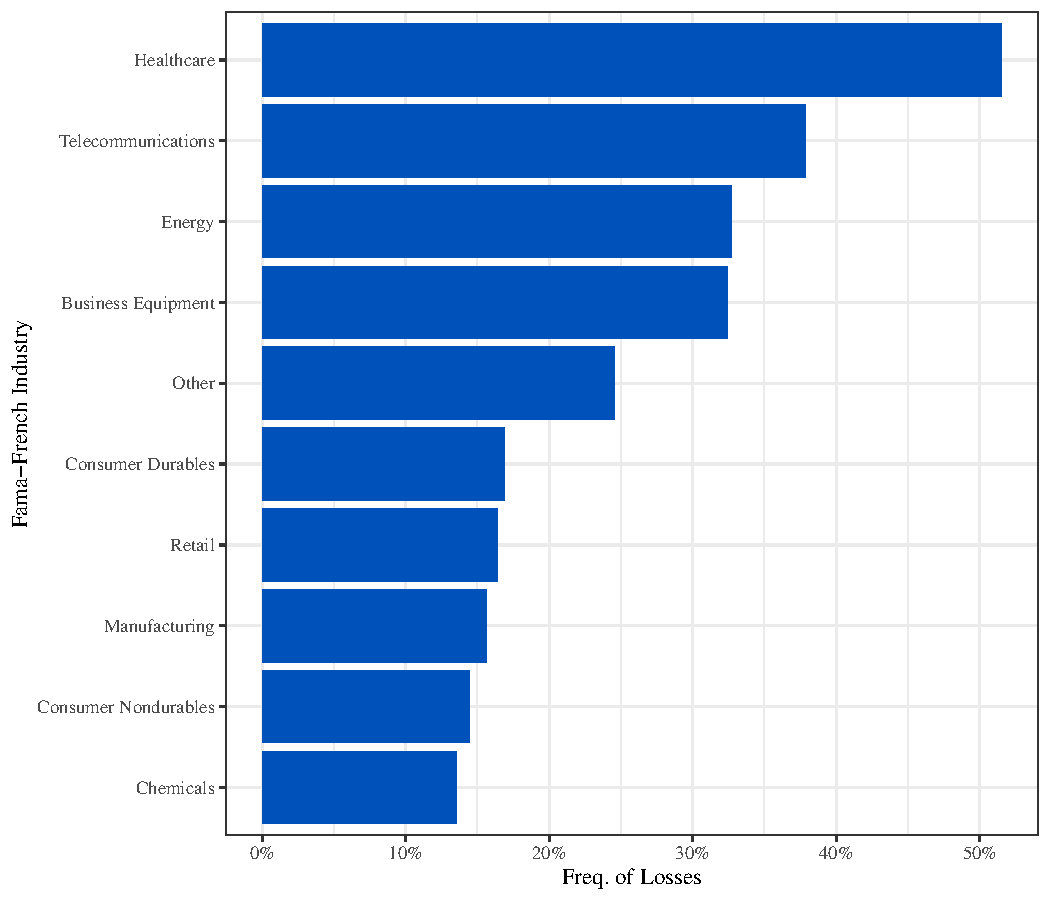
\includegraphics[scale=0.80]{figures/ff12_fig.pdf}
\footnotesize
\begin{minipage}{16cm}
\begin{singlespace}
This figure presents the frequency of SameSign (quarters where the earnings change and sales change move in the same direction) by Fama-French 12 industry classification. Figures were produced using ggplot2 (R) or plotnine (Python).
\end{singlespace}
\end{minipage}
\end{center}
\end{figure}

\clearpage\newpage

% FIGURE 2: SameSign over time + ERC by year
\begin{figure}[h!t!b]
\captionsetup{font=normal}
\caption{\textbf{Time Series}}%
\label{fig:yearly}%
\centering
\subfloat[SameSign Frequency by Size Quintile Over Time]{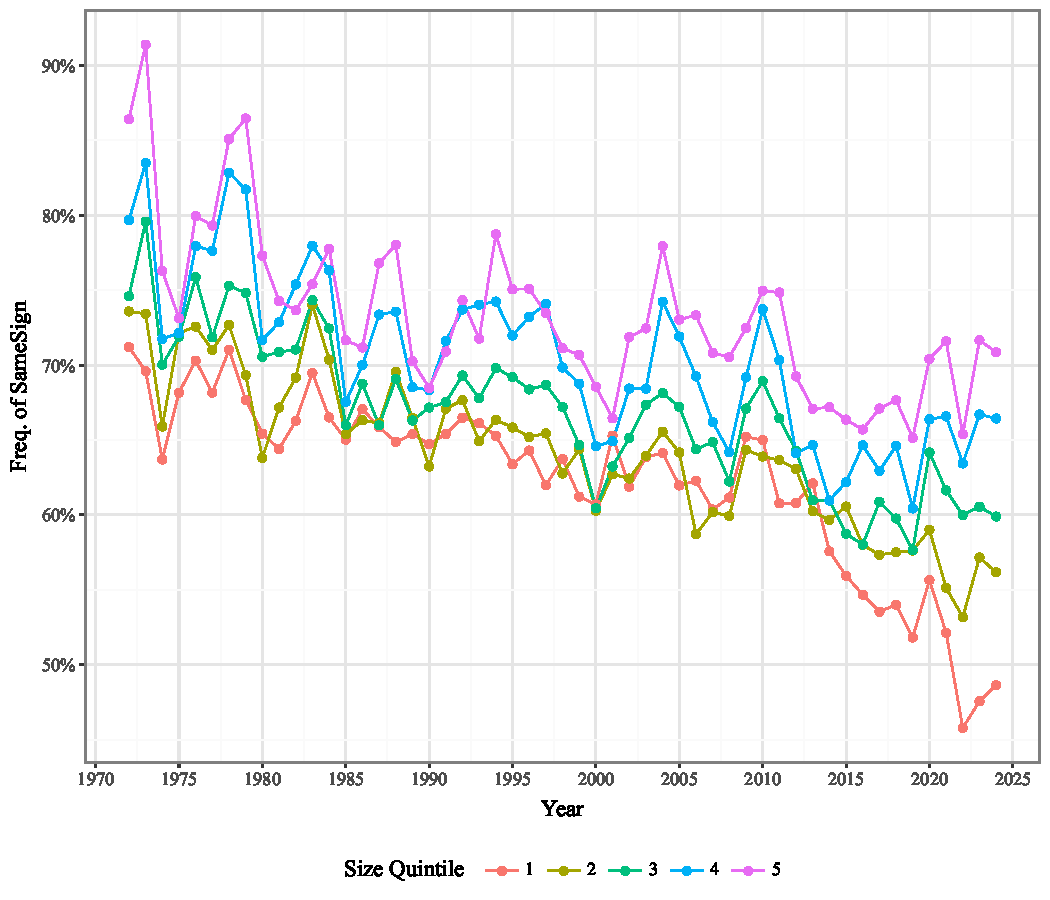
\includegraphics[width=0.48\textwidth]{figures/size_year.pdf}}\hfill
\subfloat[Year-by-Year ERC with Confidence Bands]{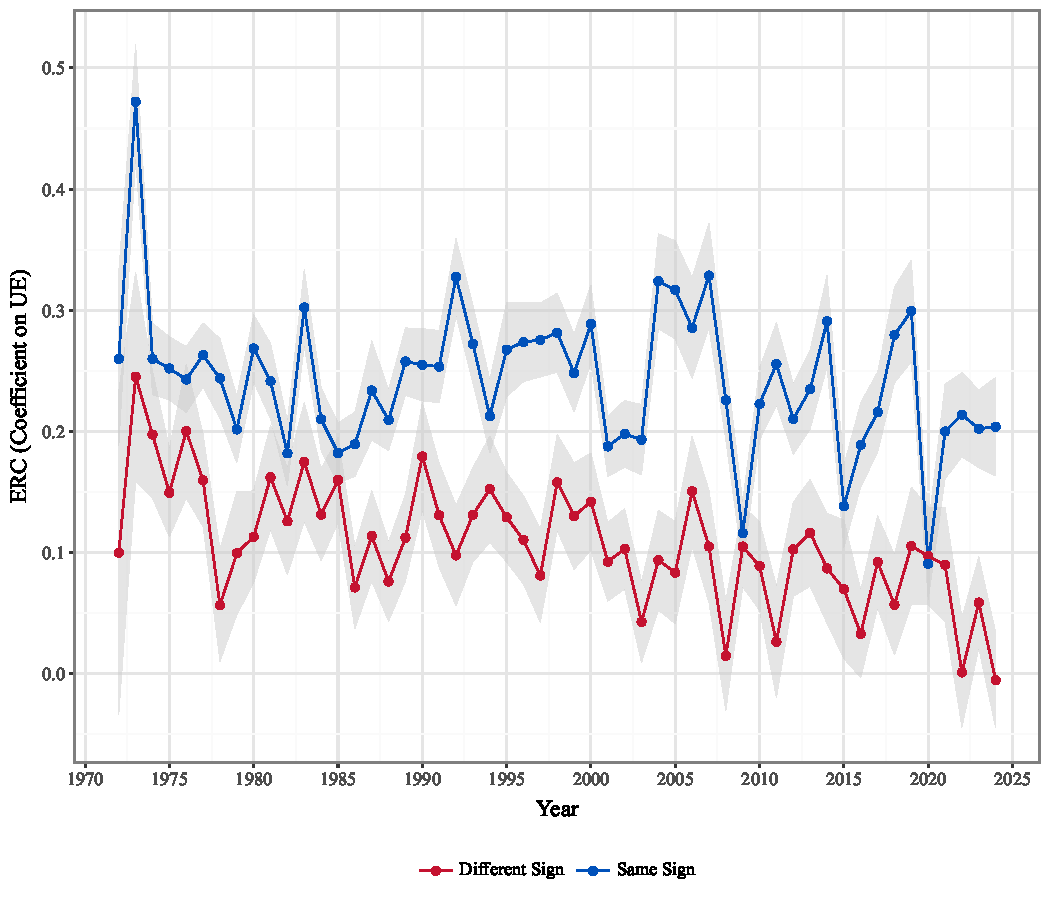
\includegraphics[width=0.48\textwidth]{figures/erc_year.pdf}}%
\footnotesize
\begin{minipage}{15.5cm}
\begin{singlespace}
\vspace{-0.3in}
Panel A plots the frequency of SameSign by market value quintile over time. Panel B plots the earnings response coefficient (ERC) --- the slope of BHAR on SUE --- estimated separately for each year, split by SameSign.
\end{singlespace}
\end{minipage}
\end{figure}

\clearpage\newpage

% FIGURE 3: Event Study CAR
\begin{figure}[h!tb]
\captionsetup{font=normal}
\caption{\textbf{Cumulative Abnormal Returns Around Earnings Announcements}}\label{fig:car}
\begin{center}
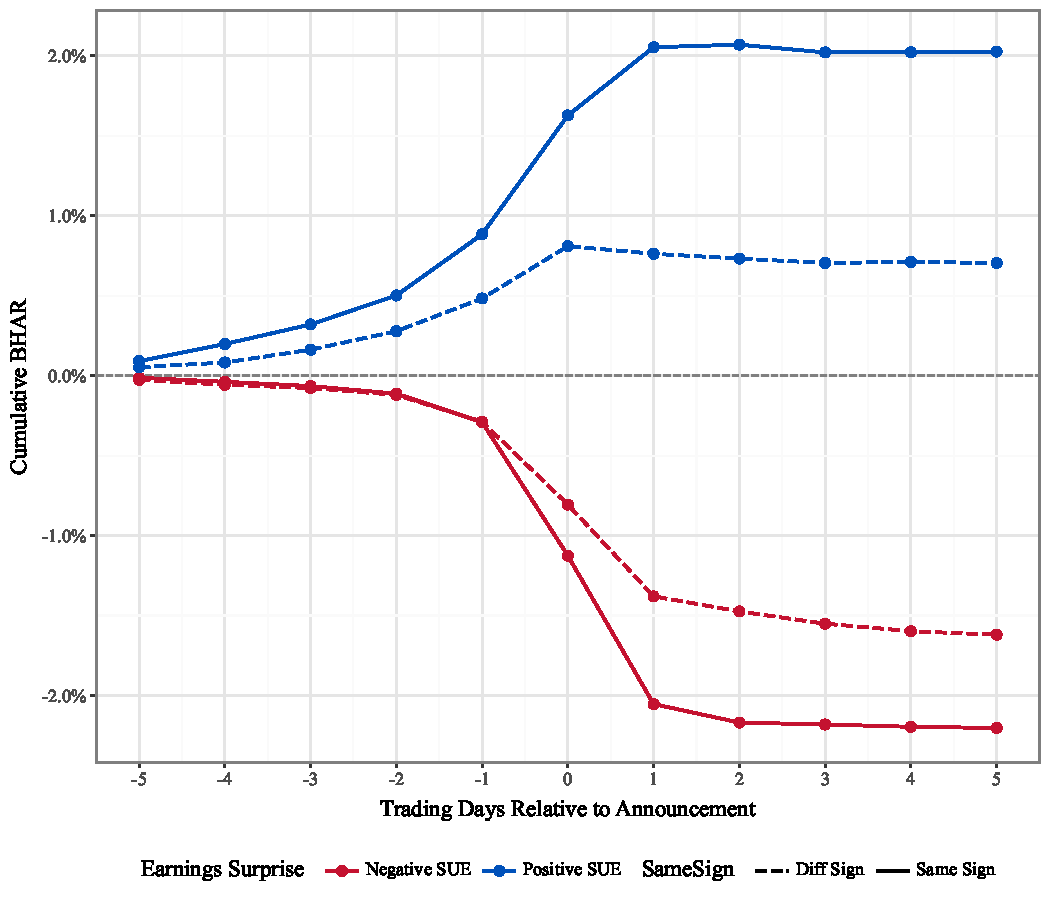
\includegraphics[scale=0.80]{figures/car_fig.pdf}
\footnotesize
\begin{minipage}{16cm}
\begin{singlespace}
This figure presents cumulative buy-and-hold abnormal returns (BHARs) over the $[-5,+5]$ trading-day window around earnings announcements, split by SUE direction (positive vs.\ negative) and SameSign (solid = same sign, dashed = different sign).
\end{singlespace}
\end{minipage}
\end{center}
\end{figure}

\clearpage\newpage


%%%%%%%%%%%%%%%%%%%%%%%%%%%%%%%%%%%%%%%%%%%%%%%%%%%%%%%%%%%%%%%%%%%%%%%%%%%%
% TABLE 1: Sample Selection
%%%%%%%%%%%%%%%%%%%%%%%%%%%%%%%%%%%%%%%%%%%%%%%%%%%%%%%%%%%%%%%%%%%%%%%%%%%%

% NOTE: This table is formatted manually for publication quality.
% The numbers come from the sample selection tracker in script 2
% (see sample-selection-r.tex or sample-selection-py.tex in the output folder).
% Update the numbers below when the pipeline is re-run.

\begin{table}[htbp]\centering\footnotesize\setstretch{1}{
\caption{\textbf{Sample Selection} \label{tab:sample-selection}}
\begin{tabular}{p{0.20in} p{4.5in} p{0.55in} p{0.65in}}
\toprule
\underline{Step} & \underline{Description} & \multicolumn{1}{c}{\underline{Obs}} & \multicolumn{1}{c}{\underline{(Diff)}}\\
1 & Compustat fundq quarterly observations with non-missing earnings announcement dates (rdq), fiscal years 1970--2024. & \multicolumn{1}{r}{1,346,387} &  \\
2 & Less: Obs in fiscal-year-change duplicates (multiple rows per gvkey $\times$ fyearq $\times$ fqtr). & \multicolumn{1}{r}{1,344,705} & \multicolumn{1}{r}{(1,682)} \\
3 & Less: Obs in gvkey $\times$ datadate duplicates. & \multicolumn{1}{r}{1,343,627} & \multicolumn{1}{r}{(1,078)} \\
4 & Less: Obs without a valid CCM link to CRSP permno. & \multicolumn{1}{r}{995,937} & \multicolumn{1}{r}{(347,690)} \\
5 & Less: Obs with duplicate permno $\times$ rdq (kept most recent fiscal quarter). & \multicolumn{1}{r}{993,116} & \multicolumn{1}{r}{(2,821)} \\
6 & Less: Obs without CRSP SIC code, or in financial (SIC 60--69) or utility (SIC 49) industries. & \multicolumn{1}{r}{769,606} & \multicolumn{1}{r}{(223,510)} \\
7 & Less: Obs without a valid seasonal lag (missing same-quarter-prior-year data or non-12-month gap). & \multicolumn{1}{r}{677,278} & \multicolumn{1}{r}{(92,328)} \\
8 & Less: Penny stocks (prior-quarter share price $\leq$ \$1). & \multicolumn{1}{r}{637,265} & \multicolumn{1}{r}{(40,013)} \\
9 & Less: Obs with missing data required for the regression (SUE, SameSign, market value, or incomplete $[-1,+1]$ BHAR window). & \multicolumn{1}{r}{617,494} & \multicolumn{1}{r}{(19,771)} \\

 & \textbf{Regression Sample} & \multicolumn{1}{r}{\textbf{617,494}} & \\
\bottomrule
\end{tabular}
}

\vspace{-1.2cm}
\singlespace
\footnotesize
\flushleft
\resizebox{\linewidth}{!}{%
\begin{tabular}{p{\linewidth}}
This table outlines our sample selection procedure. The \textit{Obs} column reports the cumulative sample size remaining after each step, and the \textit{(Diff)} column reports the number of observations removed at each step. Source data is downloaded from WRDS (Compustat fundq, CRSP daily, CCM link table). See the companion GitHub repositories for the full pipeline code that produces these counts.
\end{tabular}}
\end{table}


\clearpage\newpage

%%%%%%%%%%%%%%%%%%%%%%%%%%%%%%%%%%%%%%%%%%%%%%%%%%%%%%%%%%%%%%%%%%%%%%%%%%%%
% TABLE 2: Frequency by Decade (R)
%%%%%%%%%%%%%%%%%%%%%%%%%%%%%%%%%%%%%%%%%%%%%%%%%%%%%%%%%%%%%%%%%%%%%%%%%%%%

\begin{table}[htbp]\centering\footnotesize{
\setstretch{1.0}
\renewcommand{\arraystretch}{1.5}
\caption{\textbf{SameSign Frequency by Decade (R)} \label{tab:freq-r}}

% Pasted from freqtable-r.tex
\begin{tabular}[t]{lrrr}
\toprule
Year & Firm-Quarters & SameSign Quarters & Pct. SameSign\\
\midrule
1970 - 1979 & 52,929 & 39,546 & 74.72\%\\
1980 - 1989 & 88,307 & 61,813 & 70.00\%\\
1990 - 1999 & 139,293 & 95,309 & 68.42\%\\
2000 - 2009 & 150,034 & 98,843 & 65.88\%\\
2010 - 2019 & 124,290 & 77,838 & 62.63\%\\
2020+ & 62,641 & 37,951 & 60.58\%\\
Total & 617,494 & 411,300 & 66.61\%\\
\bottomrule
\end{tabular}

\vspace{-1.5\baselineskip}
\singlespace
\flushleft
\begin{tabular}{@{}p{\linewidth}@{}}
\footnotesize
This table reports the frequency of SameSign (quarters where earnings and sales changes move in the same direction) by decade. Created using kableExtra in R.
\end{tabular}
}
\end{table}


\clearpage\newpage

%%%%%%%%%%%%%%%%%%%%%%%%%%%%%%%%%%%%%%%%%%%%%%%%%%%%%%%%%%%%%%%%%%%%%%%%%%%%
% TABLE 3: Frequency by Decade (Stata)
%%%%%%%%%%%%%%%%%%%%%%%%%%%%%%%%%%%%%%%%%%%%%%%%%%%%%%%%%%%%%%%%%%%%%%%%%%%%

\begin{table}[htbp]\centering\footnotesize{
\setstretch{1.0}
\renewcommand{\arraystretch}{1.5}
\caption{\textbf{SameSign Frequency by Decade (Stata)} \label{tab:freq-stata}}
\def\sym#1{\ifmmode^{#1}\else\(^{#1}\)\fi}

% Pasted from freqtable-stata.tex
\begin{tabularx}{\textwidth}{Xccc}
\toprule
Year & Not SameSign & SameSign & Total\\
     & (\%) & (\%) & (\%) \\
\midrule
1970 - 1979&   13,383&   39,546&   52,929\\
          &  (25.28)&  (74.72)& (100.00)\\
1980 - 1989&   26,494&   61,813&   88,307\\
          &  (30.00)&  (70.00)& (100.00)\\
1990 - 1999&   43,984&   95,309&  139,293\\
          &  (31.58)&  (68.42)& (100.00)\\
2000 - 2009&   51,191&   98,843&  150,034\\
          &  (34.12)&  (65.88)& (100.00)\\
2010 - 2019&   46,452&   77,838&  124,290\\
          &  (37.37)&  (62.63)& (100.00)\\
2020+     &   24,690&   37,951&   62,641\\
          &  (39.42)&  (60.58)& (100.00)\\
Total     &  206,194&  411,300&  617,494\\
          &  (33.39)&  (66.61)& (100.00)\\
\bottomrule
\end{tabularx}

\vspace{-1.5\baselineskip}
\singlespace
\flushleft
\begin{tabular}{@{}p{\linewidth}@{}}
\footnotesize
This table reports the frequency of SameSign by decade. Created using estout in Stata. Note the different layout compared to the R version: Stata's \texttt{estpost tabulate} produces a cross-tabulation with row percentages, while R's version reports counts and a single percentage column.
\end{tabular}
}
\end{table}


\clearpage\newpage

%%%%%%%%%%%%%%%%%%%%%%%%%%%%%%%%%%%%%%%%%%%%%%%%%%%%%%%%%%%%%%%%%%%%%%%%%%%%
% TABLE 4: Descriptive Statistics (R)
%%%%%%%%%%%%%%%%%%%%%%%%%%%%%%%%%%%%%%%%%%%%%%%%%%%%%%%%%%%%%%%%%%%%%%%%%%%%

\begin{table}[htbp]\centering\footnotesize{
\setstretch{1.0}
\renewcommand{\arraystretch}{1.5}
\caption{\textbf{Descriptive Statistics (R)} \label{tab:descrip-r}}

% Pasted from descrip-r.tex (modelsummary/tabularray format)
\begin{tblr}[]{
colspec={Q[]Q[]Q[]Q[]Q[]Q[]Q[]Q[]Q[]},
hline{2}={1-9}{solid, black, 0.05em},
hline{1}={1-9}{solid, black, 0.1em},
hline{7}={1-9}{solid, black, 0.1em},
column{1}={}{halign=l},
column{2-9}={}{halign=r},
}
& N & Mean & SD & Min & P25 & Median & P75 & Max \\
$BHAR_{[-1,+1]}$ & 617,494 & 0.001 & 0.098 & -0.990 & -0.041 & -0.001 & 0.039 & 6.395 \\
$SUE$ & 617,494 & -0.001 & 0.067 & -0.336 & -0.009 & 0.001 & 0.009 & 0.310 \\
$SameSign$ & 617,494 & 0.666 & 0.472 & 0.000 & 0.000 & 1.000 & 1.000 & 1.000 \\
$LOSS$ & 617,494 & 0.303 & 0.460 & 0.000 & 0.000 & 0.000 & 1.000 & 1.000 \\
$\ln(MVE)$ & 617,494 & 5.613 & 2.211 & 1.248 & 3.952 & 5.487 & 7.114 & 11.219 \\
\end{tblr}

\vspace{-1.5\baselineskip}
\singlespace
\flushleft
\begin{tabular}{@{}p{\linewidth}@{}}
\footnotesize
This table provides descriptive statistics for the regression sample. Variables are as defined in Appendix~\ref{vars}. Continuous variables are winsorized at the 1st and 99th percentiles. Created using datasummary from the modelsummary package in R, which produces tabularray format.
\end{tabular}
}
\end{table}


\clearpage\newpage

%%%%%%%%%%%%%%%%%%%%%%%%%%%%%%%%%%%%%%%%%%%%%%%%%%%%%%%%%%%%%%%%%%%%%%%%%%%%
% TABLE 5: Descriptive Statistics (Python)
%%%%%%%%%%%%%%%%%%%%%%%%%%%%%%%%%%%%%%%%%%%%%%%%%%%%%%%%%%%%%%%%%%%%%%%%%%%%

\begin{table}[htbp]\centering\footnotesize{
\setstretch{1.0}
\renewcommand{\arraystretch}{1.5}
\caption{\textbf{Descriptive Statistics (Python)} \label{tab:descrip-py}}

% Pasted from descrip-py.tex (great_tables format)
% NOTE: great_tables auto-escapes LaTeX special characters, so math mode
% variable names are added manually here in the Overleaf wrapper.
\begin{tabular*}{\linewidth}{@{\extracolsep{\fill}}lrrrrrrrr}
\toprule
  & N & Mean & SD & Min & P25 & Median & P75 & Max \\
\midrule\addlinespace[2.5pt]
$BHAR_{[-1,+1]}$ & 617,494 & 0.001 & 0.098 & -0.990 & -0.041 & -0.001 & 0.039 & 6.395 \\
$SUE$ & 617,494 & -0.001 & 0.067 & -0.336 & -0.009 & 0.001 & 0.009 & 0.310 \\
$SameSign$ & 617,494 & 0.666 & 0.472 & 0.000 & 0.000 & 1.000 & 1.000 & 1.000 \\
$LOSS$ & 617,494 & 0.303 & 0.460 & 0.000 & 0.000 & 0.000 & 1.000 & 1.000 \\
$\ln(MVE)$ & 617,494 & 5.613 & 2.211 & 1.248 & 3.952 & 5.487 & 7.114 & 11.219 \\
\bottomrule
\end{tabular*}

\vspace{-1.5\baselineskip}
\singlespace
\flushleft
\begin{tabular}{@{}p{\linewidth}@{}}
\footnotesize
This table provides descriptive statistics for the regression sample. Variables are as defined in Appendix~\ref{vars}. Continuous variables are winsorized at the 1st and 99th percentiles. Created using great\_tables (by Posit) in Python. Math mode variable names are added manually in the \LaTeX\ wrapper since great\_tables auto-escapes special characters.
\end{tabular}
}
\end{table}


\clearpage\newpage

%%%%%%%%%%%%%%%%%%%%%%%%%%%%%%%%%%%%%%%%%%%%%%%%%%%%%%%%%%%%%%%%%%%%%%%%%%%%
% TABLE 6: Descriptive Statistics (Stata)
%%%%%%%%%%%%%%%%%%%%%%%%%%%%%%%%%%%%%%%%%%%%%%%%%%%%%%%%%%%%%%%%%%%%%%%%%%%%

\begin{table}[htbp]\centering\footnotesize{
\setstretch{1.0}
\renewcommand{\arraystretch}{1.5}
\caption{\textbf{Descriptive Statistics (Stata)} \label{tab:descrip-stata}}

% Pasted from descrip-stata.tex (estout format, horizontal layout)
% Variable labels are added manually since Stata uses plain text labels.
\begin{tabular}{l*{1}{cccccccc}}
\toprule
                &    N&     Mean&       SD&      Min&      P25&   Median&      P75&      Max\\
\midrule
$BHAR_{[-1,+1]}$&  617,494&    0.001&    0.098&   -0.990&   -0.041&   -0.001&    0.039&    6.395\\
$SUE$           &  617,494&   -0.001&    0.067&   -0.336&   -0.009&    0.001&    0.009&    0.310\\
$SameSign$      &  617,494&    0.666&    0.472&    0.000&    0.000&    1.000&    1.000&    1.000\\
$LOSS$          &  617,494&    0.303&    0.460&    0.000&    0.000&    0.000&    1.000&    1.000\\
$\ln(MVE)$      &  617,494&    5.613&    2.211&    1.248&    3.952&    5.487&    7.114&   11.219\\
\bottomrule
\end{tabular}

\vspace{-1.5\baselineskip}
\singlespace
\flushleft
\begin{tabular}{@{}p{\linewidth}@{}}
\footnotesize
This table provides descriptive statistics for the regression sample. Variables are as defined in Appendix~\ref{vars}. Continuous variables are winsorized at the 1st and 99th percentiles. Created using estout in Stata. Note the horizontal layout --- all statistics on one row per variable --- which requires all cell specifications to be in a single quoted string in the \texttt{cells()} option.
\end{tabular}
}
\end{table}


\clearpage\newpage

%%%%%%%%%%%%%%%%%%%%%%%%%%%%%%%%%%%%%%%%%%%%%%%%%%%%%%%%%%%%%%%%%%%%%%%%%%%%
% TABLE 7: Correlation Matrix (R)
%%%%%%%%%%%%%%%%%%%%%%%%%%%%%%%%%%%%%%%%%%%%%%%%%%%%%%%%%%%%%%%%%%%%%%%%%%%%

\begin{table}[htbp]\centering\footnotesize{
\setstretch{1.0}
\renewcommand{\arraystretch}{1.5}
\caption{\textbf{Correlation Matrix (R)} \label{tab:corr-r}}

% Pasted from corrtable-r.tex (tabularray format, Pearson above / Spearman below)
\begin{tblr}[]{
colspec={Q[]Q[]Q[]Q[]Q[]Q[]},
hline{2}={1-6}{solid, black, 0.05em},
hline{1}={1-6}{solid, black, 0.1em},
hline{7}={1-6}{solid, black, 0.1em},
column{1}={}{halign=l},
column{2-6}={}{halign=r},
}
& $BHAR_{[-1,+1]}$ & $SUE$ & $SameSign$ & $LOSS$ & $\ln(MVE)$ \\
$BHAR_{[-1,+1]}$ & 1 & .12 & .06 & -.11 & -.01 \\
$SUE$ & .19 & 1 & .01 & -.25 & .02 \\
$SameSign$ & .07 & .22 & 1 & -.19 & .04 \\
$LOSS$ & -.13 & -.34 & -.19 & 1 & -.20 \\
$\ln(MVE)$ & .03 & .01 & .04 & -.20 & 1 \\
\end{tblr}

\vspace{-1.5\baselineskip}
\singlespace
\flushleft
\begin{tabular}{@{}p{\linewidth}@{}}
\footnotesize
This table provides Pearson (Spearman) correlations above (below) the diagonal. Variables are as defined in Appendix~\ref{vars}. Created using datasummary\_correlation from the modelsummary package in R.
\end{tabular}
}
\end{table}


\clearpage\newpage

%%%%%%%%%%%%%%%%%%%%%%%%%%%%%%%%%%%%%%%%%%%%%%%%%%%%%%%%%%%%%%%%%%%%%%%%%%%%
% TABLE 8: Correlation Matrix (Python)
%%%%%%%%%%%%%%%%%%%%%%%%%%%%%%%%%%%%%%%%%%%%%%%%%%%%%%%%%%%%%%%%%%%%%%%%%%%%

\begin{table}[htbp]\centering\footnotesize{
\setstretch{1.0}
\renewcommand{\arraystretch}{1.5}
\caption{\textbf{Correlation Matrix (Python)} \label{tab:corr-py}}

% Pasted from corrtable-py.tex (great_tables format, Pearson only)
% Math mode variable names added manually (great_tables auto-escapes).
\begin{tabular*}{\linewidth}{@{\extracolsep{\fill}}lrrrrr}
\toprule
  & $BHAR_{[-1,+1]}$ & $SUE$ & $SameSign$ & $LOSS$ & $\ln(MVE)$ \\
\midrule\addlinespace[2.5pt]
$BHAR_{[-1,+1]}$ & 1.000 & 0.120 & 0.056 & -0.110 & -0.008 \\
$SUE$ & 0.120 & 1.000 & 0.012 & -0.248 & 0.021 \\
$SameSign$ & 0.056 & 0.012 & 1.000 & -0.188 & 0.040 \\
$LOSS$ & -0.110 & -0.248 & -0.188 & 1.000 & -0.203 \\
$\ln(MVE)$ & -0.008 & 0.021 & 0.040 & -0.203 & 1.000 \\
\bottomrule
\end{tabular*}

\vspace{-1.5\baselineskip}
\singlespace
\flushleft
\begin{tabular}{@{}p{\linewidth}@{}}
\footnotesize
This table provides Pearson correlations. Variables are as defined in Appendix~\ref{vars}. Created using great\_tables (by Posit) in Python. Note that pandas/great\_tables produces only one correlation type (Pearson) by default, while R's modelsummary supports the Pearson-above/Spearman-below combined display natively.
\end{tabular}
}
\end{table}


\clearpage\newpage

%%%%%%%%%%%%%%%%%%%%%%%%%%%%%%%%%%%%%%%%%%%%%%%%%%%%%%%%%%%%%%%%%%%%%%%%%%%%
% TABLE 9: Correlation Matrix (Stata)
%%%%%%%%%%%%%%%%%%%%%%%%%%%%%%%%%%%%%%%%%%%%%%%%%%%%%%%%%%%%%%%%%%%%%%%%%%%%

\begin{table}[htbp]\centering\footnotesize{
\setstretch{1.0}
\renewcommand{\arraystretch}{1.5}
\caption{\textbf{Correlation Matrix (Stata)} \label{tab:corr-stata}}
\def\sym#1{\ifmmode^{#1}\else\(^{#1}\)\fi}

% Pasted from corrtable-stata.tex (estout format, lower-triangle only)
% Variable labels added manually (Stata uses raw variable names by default).
\begin{tabular}{l*{5}{c}}
\toprule
          & $BHAR_{[-1,+1]}$ & $SUE$ & $SameSign$ & $LOSS$ & $\ln(MVE)$ \\
\midrule
$BHAR_{[-1,+1]}$ & 1.000 &       &       &       &       \\
$SUE$            & 0.120 & 1.000 &       &       &       \\
$SameSign$       & 0.056 & 0.012 & 1.000 &       &       \\
$LOSS$           & -0.110 & -0.248 & -0.188 & 1.000 &       \\
$\ln(MVE)$       & -0.008 & 0.021 & 0.040 & -0.203 & 1.000 \\
\bottomrule
\end{tabular}

\vspace{-1.5\baselineskip}
\singlespace
\flushleft
\begin{tabular}{@{}p{\linewidth}@{}}
\footnotesize
This table provides Pearson correlations (lower triangle only). Variables are as defined in Appendix~\ref{vars}. Created using estpost correlate + esttab in Stata.
\end{tabular}
}
\end{table}


\clearpage\newpage

%%%%%%%%%%%%%%%%%%%%%%%%%%%%%%%%%%%%%%%%%%%%%%%%%%%%%%%%%%%%%%%%%%%%%%%%%%%%
% TABLE 10: Regression (R)
%%%%%%%%%%%%%%%%%%%%%%%%%%%%%%%%%%%%%%%%%%%%%%%%%%%%%%%%%%%%%%%%%%%%%%%%%%%%

\begin{table}[htbp]\centering\footnotesize{
\def\sym#1{\ifmmode^{#1}\else\(^{#1}\)\fi}
\setstretch{1.0}
\caption{\textbf{Regression Results (R)} \label{tab:regress-r}}

% Pasted from regression-r.tex (tabularray format from modelsummary)
\begin{tblr}[]{
colspec={Q[]Q[]Q[]Q[]Q[]Q[]},
hline{2}={1-6}{solid, black, 0.05em},
hline{8}={1-6}{solid, black, 0.05em},
hline{1}={1-6}{solid, black, 0.1em},
hline{14}={1-6}{solid, black, 0.1em},
column{2-6}={}{halign=c},
column{1}={}{halign=l},
}
& Base & Interaction & Year FE & Two-Way FE & Controls \\
$SUE$ & 0.176\sym{***} & 0.097\sym{***} & 0.096\sym{***} & 0.095\sym{***} & 0.165\sym{***} \\
& (22.252) & (11.931) & (12.222) & (12.203) & (20.427) \\
$SameSign$ &  & 0.012\sym{***} & 0.011\sym{***} & 0.011\sym{***} & 0.008\sym{***} \\
&  & (23.958) & (24.307) & (23.846) & (18.091) \\
$SUE \times SameSign$ &  & 0.128\sym{***} & 0.133\sym{***} & 0.133\sym{***} & 0.111\sym{***} \\
&  & (10.324) & (12.234) & (12.373) & (11.477) \\
Year FE &  &  & X & X & X \\
Industry FE &  &  &  & X & X \\
Controls &  &  &  &  & X \\
N & 617,494 & 617,494 & 617,494 & 617,494 & 617,494 \\
$R^2$ & 0.014 & 0.019 & 0.020 & 0.021 & 0.031 \\
$R^2$ Within &  &  & 0.019 & 0.019 & 0.030 \\
\end{tblr}

\vspace{-1.5\baselineskip}
\singlespace
\flushleft
\begin{tabular}{@{}p{\linewidth}@{}}
\footnotesize
This table reports the estimated coefficients from Eq.~(\ref{eq:regression}). Formal variable definitions are provided in Appendix~\ref{vars}. Controls include $\ln(MVE)^{std}$ and $LOSS$, each interacted with $SUE$. ***, **, * indicate (two-tailed) significance at the 1\%, 5\%, and 10\% levels, respectively. $t$-statistics in parentheses. Standard errors are clustered by firm and fiscal year-quarter. Created using fixest + modelsummary in R.
\end{tabular}
}
\end{table}


\clearpage\newpage

%%%%%%%%%%%%%%%%%%%%%%%%%%%%%%%%%%%%%%%%%%%%%%%%%%%%%%%%%%%%%%%%%%%%%%%%%%%%
% TABLE 11: Regression (Python)
%%%%%%%%%%%%%%%%%%%%%%%%%%%%%%%%%%%%%%%%%%%%%%%%%%%%%%%%%%%%%%%%%%%%%%%%%%%%

\begin{table}[htbp]\centering\footnotesize{
\def\sym#1{\ifmmode^{#1}\else\(^{#1}\)\fi}
\setstretch{1.0}
\caption{\textbf{Regression Results (Python)} \label{tab:regress-py}}

% Pasted from regression-py.tex (pyfixest etable format)
% pyfixest uses threeparttable + tabularx with makecell for coef/t-stat pairs
\begin{tabularx}{\linewidth}{@{}>{\raggedright\arraybackslash}l>{\centering\arraybackslash}X>{\centering\arraybackslash}X>{\centering\arraybackslash}X>{\centering\arraybackslash}X>{\centering\arraybackslash}X}
\toprule
 & \multicolumn{1}{c}{Base} & \multicolumn{1}{c}{Interaction} & \multicolumn{1}{c}{Year FE} & \multicolumn{1}{c}{Two-Way FE} & \multicolumn{1}{c}{Controls} \\
\cmidrule(lr){2-2} \cmidrule(lr){3-3} \cmidrule(lr){4-4} \cmidrule(lr){5-5} \cmidrule(lr){6-6}
 & (1) & (2) & (3) & (4) & (5) \\
\midrule
\addlinespace[1ex]
$SUE$ & \makecell{0.176*** \\ (22.25)} & \makecell{0.097*** \\ (11.93)} & \makecell{0.096*** \\ (12.22)} & \makecell{0.095*** \\ (12.20)} & \makecell{0.165*** \\ (20.43)} \\
\addlinespace[0.5ex]
$SameSign$ &  & \makecell{0.012*** \\ (23.96)} & \makecell{0.011*** \\ (24.31)} & \makecell{0.011*** \\ (23.85)} & \makecell{0.008*** \\ (18.09)} \\
\addlinespace[0.5ex]
$SUE$ $\times$ $SameSign$ &  & \makecell{0.128*** \\ (10.32)} & \makecell{0.133*** \\ (12.23)} & \makecell{0.133*** \\ (12.37)} & \makecell{0.111*** \\ (11.48)} \\
\addlinespace[0.5ex]
\midrule
\addlinespace[1ex]
Year FE &  &  & Yes & Yes & Yes \\
\addlinespace[0.5ex]
Industry FE &  &  &  & Yes & Yes \\
\addlinespace[0.5ex]
Controls &  &  &  &  & Yes \\
\addlinespace[0.5ex]
Observations & 617,494 & 617,494 & 617,494 & 617,494 & 617,494 \\
\addlinespace[0.5ex]
$R^2$ & 0.014 & 0.019 & 0.02 & 0.021 & 0.031 \\
\addlinespace[0.5ex]
$R^2$ Within &  &  & 0.019 & 0.019 & 0.030 \\
\bottomrule
\end{tabularx}

\vspace{-1.5\baselineskip}
\singlespace
\flushleft
\begin{tabular}{@{}p{\linewidth}@{}}
\footnotesize
This table reports the same regression as Tables~\ref{tab:regress-r} and~\ref{tab:regress-stata}, produced using pyfixest in Python. pyfixest uses R's fixest formula syntax (\texttt{"y \textasciitilde\ x | fe1 + fe2"}) and produces LaTeX via \texttt{etable(type="tex")}. Note the \texttt{makecell} format for coefficient/t-statistic pairs and the \texttt{tabularx} layout, compared to R's tabularray and Stata's standard tabular.
\end{tabular}
}
\end{table}


\clearpage\newpage

%%%%%%%%%%%%%%%%%%%%%%%%%%%%%%%%%%%%%%%%%%%%%%%%%%%%%%%%%%%%%%%%%%%%%%%%%%%%
% TABLE 12: Regression (Stata)
%%%%%%%%%%%%%%%%%%%%%%%%%%%%%%%%%%%%%%%%%%%%%%%%%%%%%%%%%%%%%%%%%%%%%%%%%%%%

\begin{table}[htbp]\centering\footnotesize{
\def\sym#1{\ifmmode^{#1}\else\(^{#1}\)\fi}
\setstretch{1.0}
\caption{\textbf{Regression Results (Stata)} \label{tab:regress-stata}}

% Pasted from regression-stata.tex (estout format)
\begin{tabular}{l*{5}{c}}
\toprule
                &\multicolumn{1}{c}{(1)}&\multicolumn{1}{c}{(2)}&\multicolumn{1}{c}{(3)}&\multicolumn{1}{c}{(4)}&\multicolumn{1}{c}{(5)}\\
                &\multicolumn{1}{c}{Base}&\multicolumn{1}{c}{Interaction}&\multicolumn{1}{c}{Year FE}&\multicolumn{1}{c}{Two-Way FE}&\multicolumn{1}{c}{Controls}\\
\midrule
SUE             &    0.176\sym{$^{***}$}&    0.097\sym{$^{***}$}&    0.096\sym{$^{***}$}&    0.095\sym{$^{***}$}&    0.165\sym{$^{***}$}\\
                &  (22.25)              &  (11.93)              &  (12.22)              &  (12.20)              &  (20.43)              \\
$SameSign$      &                       &    0.012\sym{$^{***}$}&    0.011\sym{$^{***}$}&    0.011\sym{$^{***}$}&    0.008\sym{$^{***}$}\\
                &                       &  (23.96)              &  (24.31)              &  (23.85)              &  (18.09)              \\
$SUE \times SameSign$&                       &    0.128\sym{$^{***}$}&    0.133\sym{$^{***}$}&    0.133\sym{$^{***}$}&    0.111\sym{$^{***}$}\\
                &                       &  (10.32)              &  (12.23)              &  (12.37)              &  (11.48)              \\
Year FE         &       No              &       No              &      Yes              &      Yes              &      Yes              \\
Industry FE     &       No              &       No              &       No              &      Yes              &      Yes              \\
Constant        &      Yes              &      Yes              &       No              &       No              &       No              \\
\midrule
Controls        &                       &                       &                       &                       &      Yes              \\
N               &  617,494              &  617,494              &  617,494              &  617,494              &  617,494              \\
$R^2$           &    0.014              &    0.019              &    0.020              &    0.021              &    0.031              \\
$R^2$ Within    &    0.014              &    0.019              &    0.019              &    0.019              &    0.030              \\
\bottomrule
\end{tabular}

\vspace{-1.5\baselineskip}
\singlespace
\flushleft
\begin{tabular}{@{}p{\linewidth}@{}}
\footnotesize
This table reports the same regression as Table~\ref{tab:regress-r}, produced using reghdfe + estout in Stata. Note the slightly different formatting: Stata's estout uses a different significance symbol style and includes a ``Constant'' indicator row showing which models estimate a constant term.
\end{tabular}
}
\end{table}


\end{document}
